\documentclass[UTF8]{ctexart}
\usepackage{graphicx}
\usepackage{fancyhdr}
\usepackage[inline]{enumitem}
\usepackage{listings}
\usepackage{xcolor}      %代码着色宏包
\usepackage{multirow}
\usepackage{caption}

\pagestyle{fancy}
\cfoot{\thepage}
\rhead{Haofei Hou}

\title{《计算方法》课程实验报告}
\author{侯皓斐\ 软工2003班\ U202010851}
\date{2022年4月16日}

\lstset{
	columns=fixed,       
	numbers=left,                                        % 在左侧显示行号
	numberstyle=\tiny\color{gray},                       % 设定行号格式
	frame=none,                                          % 不显示背景边框
	backgroundcolor=\color[RGB]{245,245,244},            % 设定背景颜色
	keywordstyle=\color[RGB]{40,40,255},                 % 设定关键字颜色
	numberstyle=\footnotesize\color{darkgray},           
	commentstyle=\it\color[RGB]{0,96,96},                % 设置代码注释的格式
	stringstyle=\rmfamily\slshape\color[RGB]{128,0,0},   % 设置字符串格式
	showstringspaces=false,                              % 不显示字符串中的空格
	language=c++,                                        % 设置语言
}
\begin{document}
	\maketitle
	
	感谢覃婷婷老师的辛苦教学!
	
	三角定位算法早先在航海,测量等领域发挥了重要的作用,目前也在基于卫星的全球定位系统GPS等领域大放异彩。我们在蓝桥杯算法竞赛2020年第9题的基础上考虑一个简化的两点定位问题,并将求解面积的问题转化为数值积分的问题,并通过所学知识进行求解,解决了在不同的情况下,计算可测量面积的问题。并在最后尝试推广变步长积分算法为自适应算法,取得了较好的效果。
	
	关键词:\textit{数值积分,定位算法,机械求积公式,高斯求积公式,Newton-Cotes求积公式及其复合求积法,变步长求积法,Romberg算法,自适应Simpson算法。}
	
	
	\newpage
	\tableofcontents
	\newpage
	\section{实际问题}
	科学家小蓝${}^{[1]}$来到了一个荒岛,准备对这个荒岛进行探测考察。
	
	已知荒岛是一个三角形,三个顶点的坐标分别为$(x_1, y_1), (x_2, y_2), (x_3, y_3)$。
	
	小蓝在两个位置已经安装了发射器和接收器,小蓝手中还有一个移动设备,从而使用超声波测距实现定位。其中发射器安装在坐标$(x_A, y_A)$,接收器安装在坐标$(x_B, y_B)$。小蓝的发射器和接收器可能在岛上,也可能不在岛上。
	
	小蓝的定位设备设计有些缺陷,\textbf{只有当发射器到移动设备的距离加上移动设备到接收器的距离之和小于等于$L$时,定位设备才工作正常。}
	
	尝试计算,小蓝在荒岛上可以探测到的面积有多大(精确到小数点后6位)?
	
	我们此处假设此处的坐标均为相对坐标。$L$等元素的坐标均为$km$,且保证$-1000 \leq x_1, y_1, x_2, y_2, x_3, y_3 \leq1000,-1000 \leq x_A, y_A, x_B, y_B \leq1000,  -1000  \leq L \leq1000$。
	
	当$x_A = 10, y_A = 6, x_B = 4, y_B =  12, L =  12, x_1 =  0, y_1 =  2, x_2 =  13, y_2 =  2, x_3 =  13, y_3 =  15$时,$S = 39.985946\ km^2$。其示意图如下:
	
	\begin{figure}[h]
		\centerline{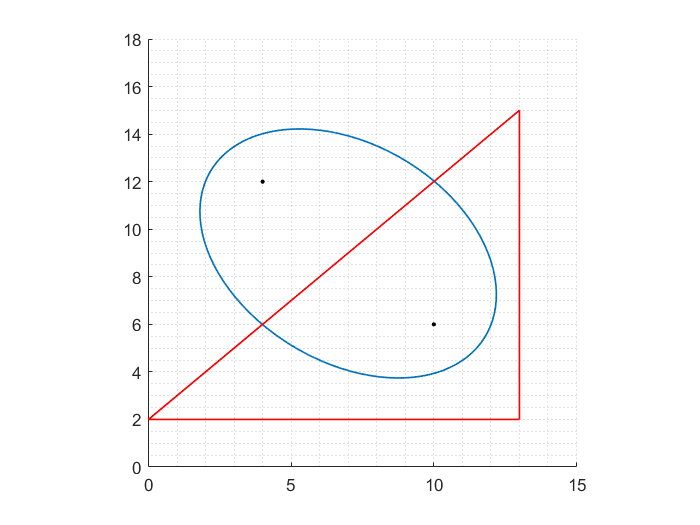
\includegraphics[width = .8\textwidth]{1.png}}
	\end{figure}
	\newpage
	\section{问题求解——数值积分}
	该实际问题可以简化为求解下面这样一个函数$f(x)$的定积分
	\[\int_{x_1}^{x_3} f(x) dx\]
	的问题。
	
	此处我们假设$x_A \leq x_B, x_1 \leq x_2, x_2 \leq x_3$。
	
	我们通过计算$x = x_0$时,
	\[\sqrt{(y-y_A)^2 + (x_0-x_A)^2} + \sqrt{(y-y_B)^2 + (x_0-x_B)^2} = L\]
	的根获得$Y_1, Y_2$。
	
	我们也计算$x = x_0$与三角形三条边的交点,获得$Y_3, Y_4$。
	
	通过多次比较获得两个图形之间在$x = x_0$时,$y$的坐标差值。	要注意各种可能的情况,并进行特判,避免出现除0等复杂的情况。
	
	\lstset{language=C++}%这条命令可以让LaTeX排版时将C++键字突出显示
	
	\begin{lstlisting}
double f (double x) {
	double C1 = L*L + (x-xB)*(x-xB) - 
	(x-xA)*(x-xA) + yB*yB - yA*yA;
	double C2 = 4*L*L*((x-xB)*(x-xB) + yB*yB);
	double k1 = 2*(yA - yB);
	double a = 4*L*L - k1*k1;
	double b = -8*L*L*yB - 2*k1*C1;
	double c = C2 - C1*C1;
	double delta = b*b - 4*a*c;
	if(delta < 0)		return 0;
	double Y1 = (-b + sqrt(delta)) / (2*a), 
	Y2 = (-b - sqrt(delta)) / (2*a);
	if(Y1 > Y2)		swap(Y1, Y2);
	double Y3 = 0, Y4 = 0, 
	Y5 = 2000, Y6 = 2000, Y7 = 2000;
	bool haveans = 0;
	if(x1 <= x && x <= x2) {
		if(x1 == x2)
		Y3 = (double)min(yy1, y2), 
		Y4 = (double)max(yy1, y2),
		haveans = 1;
		else 
		Y5 = (double)(y2-yy1) / 
		(x2-x1) * (x-x1) + yy1;
	}
	if(x2 <= x && x <= x3) {
		if(x2 == x3)
		Y3 = (double)min(y2, y3), 
		Y4 = (double)max(y2, y3),
		haveans = 1;
		else 
		Y6 = (double)(y3-y2) / 
		(x3-x2) * (x-x2) + y2;
	}
	if(x1 <= x && x <= x3) {
		if(x1 == x3)
		Y3 = (double)min(yy1, y3),
		Y4 = (double)max(yy1, y3),
		haveans = 1;
		else 
		Y7 = (double)(y3-yy1) / 
		(x3-x1) * (x-x1) + yy1;
	}
	if(haveans == 0) {
		Y3 = 2000;
		Y3 = min(Y3, Y5);
		Y3 = min(Y3, Y6);
		Y3 = min(Y3, Y7);
	} 
	if(haveans == 0) {
		Y4 = -2000;
		if(Y5 != 2000) 	Y4 = max(Y4, Y5);
		if(Y6 != 2000) 	Y4 = max(Y4, Y6);
		if(Y7 != 2000) 	Y4 = max(Y4, Y7);
	} 
	if(Y3 > Y4)		return 0;
	double Yy = max(Y1, Y3);
	double Yx = min(Y2, Y4);
	return Yx - Yy > 0? Yx - Yy:0;
}
	\end{lstlisting}
	
	此函数由于表达式未知,且判断的情况极度复杂,难以用数学方法获得其解析解。下面我们用多种方法求解此数值积分问题,并对结果进行分析。
	
	\subsection{机械求积公式与Gauss求积公式}
	
	\subsubsection{设计与编程实现}
	为了便于编程实现,我们考虑使用具有等距节点的插值型求积公式(即Newton-Cotes求积公式)和Gauss公式进行计算。
	
	我们使用$N+1$个插值节点的Newton-Cotes公式至少具有$N$次代数精度。($N$为偶数时,Newton-Cotes公式至少具有$N+1$次代数精度)。而具有$N+1$个插值节点的Gauss求积公式具有$2N+1$次代数精度。
	
	而Newton-Cotes公式的Cotes系数可以通过\textbf{代数精度法}提前求解出并打入程序直接使用。而Gauss公式中使用的Gauss点与系数较为复杂,$N \geq 3$的后的Gauss公式难以手工构造,所以我们可借助网络等方式获得Gauss点与系数打入程序直接使用。
	
	Newton-Cotes公式计算积分的代码如下:
	\lstset{language=C++}%这条命令可以让LaTeX排版时将C++键字突出显示
	
	\begin{lstlisting}
//	Newton-Cotes法
double C[8][9] = { {}, {2, 1,1}, {6, 1, 4,1}, 
	{8, 1, 3,3,1}, {90, 7, 32, 12,32,7}, 
	{288, 19, 75, 50,50,75,19}, 
	{840, 41, 216, 27, 272,27,216,41},
	{17280,751,3577,1323,2989,2989,1323,3577,751} 
};//Cotes系数
double Newton_Cotes(double a, double b) {
	//[a, b]为积分上下限
	for(int N = 1; N <= 7; N++) {
		double h = (b - a) / N;
		double sum = 0;
		for (int n = 0; n <= N+1; n++) 
			sum += C[N][n] * f(a + h*n);
		sum = sum / C[N][0] * (b - a);
		printf("N = %d, ans = %0.6lf\n", N, sum);
	}
}		
	\end{lstlisting}

	Gauss公式计算积分的代码如下:
\lstset{language=C++}%这条命令可以让LaTeX排版时将C++键字突出显示

\begin{lstlisting}
//	Gauss法
void Gauss(double a, double b) {
	//[a, b]为积分上下限
	double k = (b-a)/2, v = (a+b)/2;
	for(int N = 1; N <= 7; N++) {
		init(N);
		double sum = 0;
		for(int n = 0; n <= N+1; n++)
			sum += A[n] * f(k * X[n] + v);
		sum = sum * (b-a)/2;
		printf("N = %d, ans = %0.6lf\n", N, sum);
	}
}
\end{lstlisting}
	
	\subsubsection{计算结果}	
	计算结果如下表:
	\begin{center}
		\begin{tabular}{ |c|c|c|c|c|c|c| } 
			\hline
			\multirow{2}{1em}{$N$}  & \multicolumn{3}{|c|}{Newton-Cotes} & \multicolumn{3}{|c|}{Gauss} \\ \cline{2-7} 
			& 值 & 误差 & 代数精度 & 值 & 误差 & 代数精度 \\ \hline
			1 & 0.000000 & 39.985946 & 1 & 49.664527 & 9.678581 & 3 \\ \hline
			2 & 9.120756 & 30.865190 & 2 & 41.594896 & 1.608950 & 5 \\ \hline
			3 & 34.508763 & 5.477183 & 3 & 35.975708 & 4.010238 & 7 \\ \hline
			4 & 33.018036 & 6.967910 & 4 & 40.454571 & 0.468625 & 9 \\ \hline
			5 & 37.487880 & 2.498066 & 5 & 39.907428 & 0.078518 & 11 \\ \hline
			6 & 35.580029 & 4.405917 & 6 & 39.492366 & 0.493580 & 13 \\ \hline
			7 & 37.688346 & 2.297600 & 7 & 41.581639 & 1.595693 & 15 \\
			\hline
		\end{tabular}
	\end{center}

	\subsubsection{误差分析}
	
	绝对误差随$N$的关系如下图:
	
	\begin{figure}[h]
		\centerline{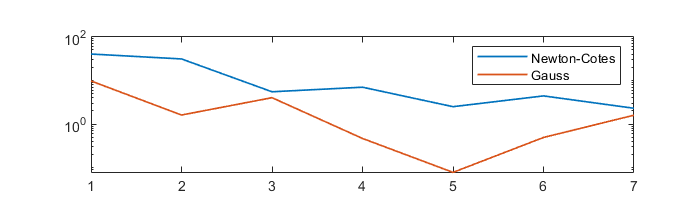
\includegraphics[width = \textwidth]{3.png}}
	\end{figure}

	Newton-Cotes公式的理论计算误差为
	\[ R(f) = Kf^{(m+1)}(\eta)\]
	其中$m$为公式的代数精度。$K$满足$K \dot (m+1)! = \frac{b^{m+2}-a^{m+2}}{m+2} - \sum_{n=0}^{N}A_nx_n^{m+1}$。
	
	而我们的被积分的函数$f(x)$无法写出具体的表达式,更难以判断其可导性,故难以从理论的角度分析其误差上限。
	
	但我们可以从图中了解到一些性质。Newton-Cotes公式和Gauss公式在$N$较小时,其误差较大,其主要原因应该是$f(x)$在端点处有着零值,随着插值节点数的增加,这一段造成的误差减少。但是当$N \geq 5$后Newton-Cotes公式误差震荡减小,减小误差提升小,其原因可能是在高阶情况下,其稳定性降低,产生了较大的误差。而Gauss公式稳定性好,且由于其精度高,计算误差小。随$N$趋向于无穷大,答案趋向于真实值。
	
	\subsection{Newton-Cotes求积公式及其复合求积法}
	
	\subsubsection{设计与编程实现}
	我们可以轻松的分析出,函数应该是分段的函数,每一段上可能是线性函数,可能是一个复杂的隐函数。而这个隐函数应该是由椭圆的方程与直线组合而成,椭圆标准方程为二次型,故这个函数阶数不高于二次,应该能在使用复合梯形公式和复合Simpson公式的情况下求出误差较低的解,而高阶的Newton-Cotes公式反而可能由于Runge现象,误差增大。
	
	我们把区间$[a, b]$等分为$N$个子区间。然后在每个子区间上用复合梯形公式和复合Simpson公式。
	
	复合求积法的代码如下:
	\lstset{language=C++}%这条命令可以让LaTeX排版时将C++键字突出显示
	
	\begin{lstlisting}
double CompositeIntegrationRule(double a, double b,
int N, string NC) {
	//[a, b]为积分上下限,N为分段次数
	//NC表示采用的复合求积公式
	if(NC == "trapezium") {
		double h = (b-a)/N;
		double sum = 0;
		for(int n = 0; n <= N-1; n++)
		sum += h*(f(a + h*n) + f(a + h*(n+1)))/2;
		return sum;
	}	
	else if (NC == "simpson") {
		double h = (b-a)/N;
		double sum = 0;
		for(int n = 0; n <= N-1; n++)
		sum += h*(f(a + h*n) + 
			4*f(a + h*(n+0.5)) 
			+ f(a + h*(n+1)))/6;
		return sum;
	}					
}
	\end{lstlisting}
	\subsubsection{计算结果}
	\begin{center}
		\begin{tabular}{ |c|c|c| } 
			\hline
			$N$  & trapezium & simpson \\ \hline
			1&0.000000&36.483023\\\hline
			10&40.535418&39.506691\\\hline
			100&39.963369&39.995587\\\hline
			1000&39.986579&39.986128\\\hline
			10000&39.985946&39.985959\\\hline
			100000&39.985947&39.985946\\\hline
			1000000&39.985946&39.985946\\\hline
		\end{tabular}
	\end{center}
	\subsubsection{误差分析}
	\begin{figure}[h]
		\centerline{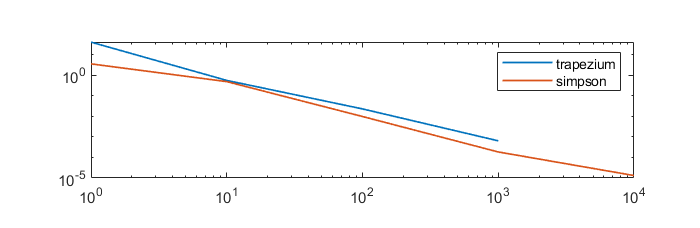
\includegraphics[width = \textwidth]{4.png}}
	\end{figure}
	从图表中容易看出,复合梯形公式首先在小数点后6位接近真实值。但是其稳定性不及复合Simpson公式,当$N = 10^5$时反而误差增大。两个公式均在迭代$N = 10^5$次取得了较好的效果。
	
	而且随着$N$的增大,其误差水平显著降低。可从simpson公式的余项中可见一斑。
	\[\tilde{R}_s(f)=-\frac{h^4}{2880}[f^{(3)}(b) - f^{(3)}(a)]\]
	随着$N$的增大,$h$以反比的速度减小,最大误差以四次方反比的速度减小。取得了好的计算效果的同时,增加了计算的时间代价。
	\subsection{变步长求积法与Romberg算法}
	
	\subsubsection{设计与编程实现}
	
	我们为了精确的求出复合误差要求$eps \leq 10^{-7}$的数值解,使用变步长求积法与Romberg算法。
	
	我们可将朴素的变步长求积法视为外推0次的Romberg算法,我们尝试外推$l = 0, 1, 2, 3, 4, 5$次。每外推一次即相当于增大了每个步长内求积公式的阶数。外推次数过多时,稳定性降低,计算误差增大。
	
		\lstset{language=C++}%这条命令可以让LaTeX排版时将C++键字突出显示
	
	\begin{lstlisting}
void asr(double a, double b, int l) {
double T[6][2000];
//[a, b]为积分上下限,l为外推次数
T[0][0] = (b - a) / 2 * (f(a) + f(b));
for(int m = 0; m <= l; m++)
for(int i = 0; i <= l-m; i++) {
if(m == 0) {
	if(i == 0)	continue; 
	T[0][i] = T[0][i-1]/2;
	for(int j = 1; j <= (1<<(i - 1)); j++) 
	T[0][i] += ((b - a) / (double)(1 << i)) * 
	f(a+(((double)(2*j-1)/(1 << i))*(b - a)));				
}
else 
	T[m][i] = ((1<<(2*m) *T[m-1][i+1] - T[m-1][i])/
	((1 << (2*m)) - 1);
}
for(int i = 1; ; i++) {
	T[0][i+l] = T[0][i+l-1]/2;
	for(int j = 1; j <= (1<<(i+l - 1)); j++) 
	T[0][i+l] += (b - a) / (double)(1 << (i+l)) * 
	f(a + ((double)(2*j-1)/(1<<(i+l))*(b - a)));
	for(int m = 1; m <= l; m++)
	T[m][i+l-m] = ((1 << (2*m)) * T[m-1][i+l-m+1]-
	T[m-1][i+l-m])/((1 << (2*m)) - 1);
	if(abs(T[l][i] - T[l][i-1]) < eps) {
		printf("%0.6lf\n", T[l][i]);
		return ;
	}
}	
	\end{lstlisting}

	\subsubsection{计算结果}
		\begin{center}
		\begin{tabular}{ |c|c|c|c| } 
			\hline
			$l$  & 计算结果 & 变步长次数 & 计算时间 \\ \hline
			0&39.985946&21&0.060000\\\hline
			1&39.985946&21&0.109000\\\hline
			2&39.985946&21&0.107000\\\hline
			3&39.985946&21&0.109000\\\hline
			4&39.985946&21&0.108000\\\hline
			5&39.985946&21&0.111000\\\hline
		\end{tabular}
	\end{center}
	
	我们由变步长梯形求积公式的事后误差估计公式
	\[I - T_{k+1} \approx \frac{1}{3}(T_{k+1}-T_{k})\]
	由于上式是一个近似估计,我们保守的使$T_{k+1}-T_{k}$作为Romberg算法的计算误差,并使$T_{k+1}-T_{k}\leq \frac{eps}{10}$,可以保证计算得出满足误差要求的数值解。
	
	\begin{figure}[h]
		\centerline{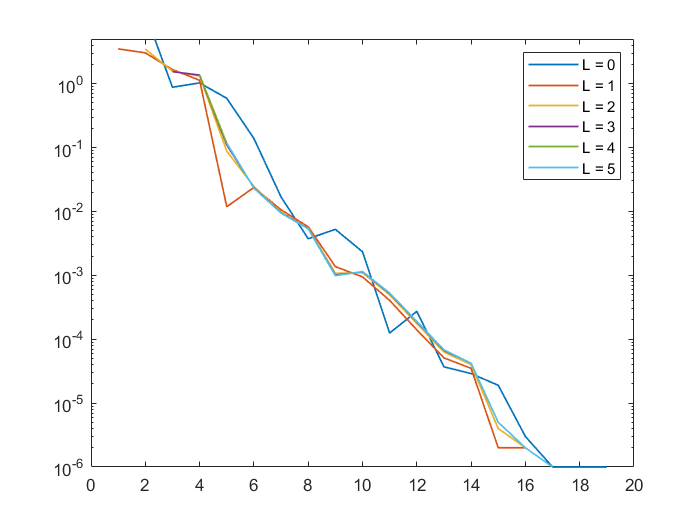
\includegraphics[width = 0.8\textwidth]{5.png}}
		\caption*{步长衰减与绝对误差的关系示意图}
	\end{figure}
	
	\subsubsection{计算效率分析}
	
	从表中可以看出,随着外推次数的增多,计算速度和收敛情况并未有更优化,反而增大了计算的时间。这也可能和本积分特殊的性质有关系。\footnote{可见2.2.1的相关分析}
	
	从上图(步长衰减与绝对误差的关系示意图)中可以看出随着外推次数增加,其计算误差曲线更加平滑,稳定性更好。实际计算中应该取外推次数$l = 2$为宜。
	
	\section{算法对比分析}
	
	机械求积公式与Gauss求积公式在编程实现中难以推向高阶,但在低阶的情况下计算简单,清晰。也有着不错的效果,可以迅速估算出一个定积分的大概的取值。若是表达式已知的情况下还可以进行简单的误差分析。高阶Newton-Cotes公式可能会出现较强的Runge现象,造成稳定性不佳。
	
	利用Newton-Cotes求积公式及其复合求积法,可以获得较好的计算精度,但其在本问题的情况下难以进行事先误差分析,分段数量$N$不能提前确定,为达到较好的精度需要多次尝试。该算法计算量较大。
	
	变步长求积法与Romberg算法的实现较为复杂,但结果比较优秀,可以自适应的确定计算的节点分段次数并达到想要的误差精度。而且Romberg算法计算时间和耗费的计算资源都相当多。在本题中外推并未显著的提升计算的精度,但对于计算的稳定性提升有着较好的帮助,最后确定适合本问题的外推次数应该为$l = 2$。
	
	在解决此类数值积分问题时,由于我们的目标是获得相对精确的数值解,Romberg算法应该是最优的选择。我们也可以\textbf{对Romberg算法进行一定的改造,减少其计算量}。其思想是:当再次分段后的数值解若与分段前的数值解的后验误差$\leq \frac{eps}{10}$后,便在这一个区间停止分段。最经典的实现应该为\textbf{自适应Simpson算法}${}^{[2]}$。在本实验中Romberg算法外推1次的情况下,为达到计算精度,计算时间为0.109000s,笔者用C++实现的自适应Simpson算法仅需0.001000s。
	
	\newpage
	
	\section{实验结论}
	
	我们可以确定回答小蓝,他能够探索的范围面积$S = 39.985946\ km^2$。
	
	该代码可扩展性强,由于$f(x)$代码实现得当,在其他复杂的岛屿地理情况下仍能具有可移植性。
	
	此问题也有着可扩展的空间,任意图形的相交区域的面积的求解只需要对函数$f(x)$进行修改。
	
	而实际上,两个点可以在平面上确认两个点。当我们增加一个固定的测距仪器时便可以实现精确的定位,此时也会出现定位范围问题。而当拥有四个固定的测距仪器时,我们便可以确定三维空间中点的坐标位置。因此这个问题具有着非常深入的意义,GPS定位系统中如何确定卫星的坐标从而使得卫星可覆盖的面积最大?这些问题可能会基于本文这个简陋的模型。${}^{[3]}$
	
	\section{致谢}
	感谢覃婷婷老师的教学!覃婷婷老师是认真负责,严谨细致的华中科技大学数学学者的杰出代表。
	
	难以忘记覃婷婷与助教老师每次细致的批改,而且提供了大量的资料帮助同学学习与理解。覃婷婷老师上课注重知识的来源与发现的思维过程,而不是拘泥于每一个算法的具体实现和数学背景,确实是提升了我们的视野!覃婷婷老师教材与PPT的配合详略得当,充分便于同学自学以及备考,而且作业题也紧跟课程,简单而有深度。
	\section{参考资料}
	
	本文章的模型基于2020年第十一届蓝桥杯算法设计竞赛第9题建立。
	
		
		[1]蓝桥杯2020年第十一届省赛真题-荒岛探测(已通过全部测试点)
		
		https://www.dotcpp.com/oj/problem2573.html
		
		[2]自适应Simpson算法
		
		https://www.cnblogs.com/pks-t/p/10277958.html
		
		[3]三点定位法
		
		https://www.zhihu.com/question/22040578?sort=created
		
		[4]张诚坚,何南忠,覃婷婷.计算方法(第二版)[M].北京:高等教育出版社,2021.
		
\end{document}